\documentclass{beamer}

\usepackage[thinlines]{easytable}
\usepackage{tcolorbox}
\usepackage{cancel}
\usepackage{amsmath}
\usepackage{graphicx}

\usepackage[style=alphabetic]{biblatex}
\addbibresource{refs.bib}

\let\Im\relax
\DeclareMathOperator{\Im}{Im}

\usetheme{AnnArbor}
\usefonttheme{serif}

\title{Eigenvalue Algorithms}

\subtitle{Numerical Strategies Providing for the Time and Resource Efficient Computation of Eigenvalues for Any General Square Matrix}
\author{Jayden Li}
\date{Friday, March 7, 2025}

\begin{document}

\frame{\titlepage}

\begin{frame}
\frametitle{The Problem}

\begin{center}
	\begin{tcolorbox}[colback=yellow!5!white,colframe=yellow!75!black,parbox=false,width=0.6\linewidth]
		\centering
		How can we find the eigenvalues of any $n\times n$ matrix $A$?
		\begin{equation*}
			A\mathbf x=\lambda\mathbf x
		\end{equation*}
	\end{tcolorbox}
\end{center}

\end{frame}

\begin{frame}
	\frametitle{Table of Contents}
	\tableofcontents
\end{frame}

\section{Power Method}
\frame{\sectionpage}

\begin{frame}
	\frametitle{Power Method}
	\begin{tcolorbox}[title={Power Method},colback=red!5!white,colframe=red!75!black,parbox=false]
		\begin{enumerate}
			\item<1-> Let $x_0$ be a random vector in $\mathbb R^n$.
			\item<2-> Define $\displaystyle x_{i+1}=\frac{Ax_i}{||Ax_i||}$. Then $x_k\neq A^kx_0$, but are pointing in the same direction.
			\item<3-> Iterate the above process for $m$ steps. Now, we have have calculated $x_m$, which is parallel to $A^m x_0$.
			\item<4-> Calculate the dominant eigenvalue $\displaystyle \lambda_1=\frac{\left\Vert A A^m x_0 \right\Vert}{\left\Vert A^m x_0 \right\Vert}=\frac{\left\Vert A x_m\right\Vert}{\left\Vert x_m \right\Vert}=\frac{Ax_m\cdot x_m}{x_m \cdot x_m}$.
		\end{enumerate}
		\onslide<4->{Reference: \cite{kochlab}.}
	\end{tcolorbox}
\end{frame}

\begin{frame}
	\frametitle{Derivation of the Power Method (1)}
	\begin{itemize}
		\item<1-> $A$ is an $n\times n$ matrix.
		\item<2-> We are basically multiplying on the left by $A$.
		\item<3-> Algorithm tends to $\displaystyle \lim_{k\to\infty}A^k x_0$.
		\item<4-> Let $A=PDP^{-1}$ be the diagonalization.
		\item<4-> Then $\displaystyle \lim_{k\to\infty}A^k=PD^kP^{-1}$.
		\item<5-> $\displaystyle \lim_{k\to\infty}A^kP=PD^k$.
	\end{itemize}
\end{frame}

\begin{frame}
	\frametitle{Derivation of the Power Method (2)}
	\begin{itemize}
		\item<1-> Let $\left|\lambda_1\right|\geq \left|\lambda_2\right|\geq\ldots\geq \left|\lambda_n\right|$. The $\lambda_i$'s are eigenvalues of $A$.
		\item<2-> Quick reminder: $D$ is diagonal matrix of eigenvalues.
			\begin{equation*}
				D=\begin{bmatrix}
					\lambda_1 &&& \\
					& \lambda_2 && \\
					&& \ddots & \\
					&&& \lambda_n
				\end{bmatrix}
			\end{equation*}
		\item<3-> Choose a random vector $v_0\in\mathbb R^n$, let $v=Pv_0$.
		\item<4-> $\displaystyle \lim_{k\to\infty}A^kP=PD^k$ becomes $\displaystyle \lim_{k\to\infty}A^kPv_0=PD^kv_0$.
	\end{itemize}
\end{frame}

\begin{frame}
	\frametitle{Derivation of the Power Method (3)}
	\begin{itemize}
		\item<1-> $\displaystyle \lim_{k\to\infty}A^kP=PD^k$ becomes $\displaystyle \lim_{k\to\infty}A^kPv_0=PD^kv_0=A^kv$.
		\item<2->[]
		\begin{equation*}
			A^k v 
			= P \begin{bmatrix}
				\lambda_1^k & & \\
				& \ddots & \\
				& & \lambda_n^k
			\end{bmatrix}
			\begin{bmatrix}
				v_{0_1} \\ \vdots \\ v_{0_n}
			\end{bmatrix}
			=\begin{bmatrix}
				p_1 & \ldots & p_n
			\end{bmatrix} \begin{bmatrix}
				\lambda_1^k v_{0_1} \\ 
				\vdots \\
				\lambda_n^k v_{0_n} \\ 
			\end{bmatrix}
		\end{equation*}

		\item<3->[]
		\begin{equation*}
			A^kv=\sum_{i=1}^{n}\lambda_i^k v_{0_i} p_i
			=\sum_{i=1}^{n}\lambda_1^k\frac{\lambda_i^k}{\lambda_1^k} v_{0_i} p_i
			=\lambda_1^k \sum_{i=1}^{n}\left(\frac{\lambda_i}{\lambda_1}\right)^k v_{0_i}p_i
		\end{equation*}
	
		\item<4->
		Now, if $\left|\lambda_1\right|>\left|\lambda_2\right|\geq\ldots\geq \left|\lambda_n\right|$, then $\lambda_i/\lambda_1<1$ for all $i\neq 1$.
		\begin{equation*}
		    A^kv=\lambda_1^k v_{0_1}p_1
		\end{equation*}

		\item<5-> $A^k$ is an eigenvector of $A$.
	\end{itemize}
\end{frame}

\begin{frame}
	\frametitle{Derivation of the Power Method (4)}
	\begin{itemize}
		\item<1-> Now suppose $\left|\lambda_1\right|=\left|\lambda_2\right|$.
		\item<2->[]
		\begin{equation*}
			A^kv=\sum_{i=1}^{n}\lambda_i^k v_{0_i} p_i
			=\sum_{i=1}^{n}\lambda_1^k\frac{\lambda_i^k}{\lambda_1^k} v_{0_i} p_i
			=\lambda_1^k \sum_{i=1}^{n}\left(\frac{\lambda_i}{\lambda_1}\right)^k v_{0_i}p_i
		\end{equation*}
		\item<2->[]
		\begin{equation*}
			A^k v
			=\lim_{k\to\infty}\lambda_1^k \left(\cancel{\left(\frac{\lambda_1}{\lambda_1}\right)^k} v_{0_1}p_1+\cancel{\left(\frac{\lambda_2}{\lambda_1}\right)^k}v_{0_2}p_2+\cancel{\sum_{i=3}^{n}\left(\frac{\lambda_i}{\lambda_1}\right)^k v_{0_i}p_i}\right)
		\end{equation*}
		\item<2->[]
		\begin{equation*}
			A^k v
			=\lim_{k\to\infty}\lambda_1^k\left(v_{0_1}p_1+v_{0_2}p_2\right)
		\end{equation*}
		is not an eigenvector of $A$ if $\lambda_1\neq\lambda_2$.
	\end{itemize}
\end{frame}

\begin{frame}
	\frametitle{Problems with the Power Method}
	\begin{itemize}
		\item<1-> If $\left|\lambda_1\right|=\left|\lambda_2\right|$, then $(\lambda_1/\lambda_2)^k$ tends to $1$, not $0$.
		\item<2-> If dominant eigenvalue $\lambda_1=a+bi$ is complex ($b\neq0$), then $\lambda_2=\overline{\lambda_1}=a-bi$ is also eigenvalue.
		\item<3-> But $\left|\lambda_1\right|=\sqrt{a^2+b^2}=\left|\lambda_2\right|$.
		\item<4-> Cannot calculate complex eigenvalues.
		\item<5-> Can use shifts (calculate eigenvalues of $A-cI$), but that is complicated.
		\item<6-> Even worse: only calculates dominant eigenvalue.
		\item<7-> Speed of convergence depends on choice of starting vector.
	\end{itemize}
\end{frame}

\section{Basic $QR$ Algorithm}
\frame{\sectionpage}

\begin{frame}
	\frametitle{Basic $QR$ Algorithm}
	\begin{tcolorbox}[title={Schur form},colback=blue!5!white,colframe=blue!75!black,parbox=false]
		Let $A$ be an $n\times n$ real matrix. The \textbf{Schur form} of $A$ is:
		\begin{equation*}
			A=QUQ^T=QUQ^{-1}
		\end{equation*}
		where $Q$ is orthogonal and $U$ is upper triangular. $A$ and $U$ are similar so they share the same eigenvalues, which are the diagonal entries of $U$.
	\end{tcolorbox}
\end{frame}

\begin{frame}
	\frametitle{Basic $QR$ Algorithm}
	\begin{tcolorbox}[title={Basic $QR$ Algorithm},colback=red!5!white,colframe=red!75!black,parbox=false]
		\begin{enumerate}
			\item<1-> Set $A_1=A$.
			\item<2-> Define $A_{i+1}=R_iQ_i$, where $A_1=Q_iR_i$.
			\item<3-> Iterate step 2 $m$ times to calculate $A_{m+1}$.
			\item<4-> If ``good case,'' $A_{m+1}$ tends to a triangular matrix ($U$ in Schur form). Trivial to read off eigenvalues.
		\end{enumerate}
		\onslide<4->{Reference: \cite[64]{ethbook}.}
	\end{tcolorbox}
	\onslide<5->{Proof is hard and complicated. We will ``prove'' by example.}
\end{frame}

\begin{frame}
	\frametitle{Example of the Basic $QR$ Algorithm (1)}
	\begin{equation*}
	    A=\begin{bmatrix}
			1 & 2 & 3 \\
			4 & 5 & 6 \\
			7 & 8 & 1
	    \end{bmatrix}
	\end{equation*}
	\begin{center}
		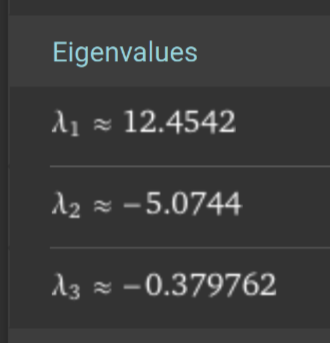
\includegraphics[width=0.4\textwidth]{eigenvalues.png}
	\end{center}
\end{frame}

\begin{frame}
	\frametitle{Example of the Basic $QR$ Algorithm (2)}
	\begin{align*}
		\onslide<1->{A_1 &= 
		\begin{bmatrix}
			1.00 & 2.00 & 3.00 \\
			4.00 & 5.00 & 6.00 \\
			7.00 & 8.00 & 1.00 \\
		\end{bmatrix}} \\
		\onslide<2->{Q_1 &= 
		\begin{bmatrix}
			-0.12 & 0.90 & 0.41 \\
			-0.49 & 0.30 & -0.82 \\
			-0.86 & -0.30 & 0.41 \\
		\end{bmatrix}} \\
		\onslide<2->{R_1 &= 
		\begin{bmatrix}
			-8.12 & -9.60 & -4.19 \\
			0.00 & 0.90 & 4.22 \\
			0.00 & 0.00 & -3.27 \\
		\end{bmatrix}} \\
		\onslide<3->{A_2 &= 
		\begin{bmatrix}
			9.33 & -8.98 & 2.81 \\
			-4.08 & -1.00 & 0.98 \\
			2.81 & 0.98 & -1.33 \\
		\end{bmatrix}}
	\end{align*}
\end{frame}

\begin{frame}
	\frametitle{Example of the Basic $QR$ Algorithm (3)}
	\begin{align*}
		\onslide<1->{A_2 &= 
		\begin{bmatrix}
			9.33 & -8.98 & 2.81 \\
			-4.08 & -1.00 & 0.98 \\
			2.81 & 0.98 & -1.33 \\
		\end{bmatrix}} \\
		\onslide<2->{Q_2 &= 
		\begin{bmatrix}
			-0.88 & -0.47 & 0.02 \\
			0.39 & -0.70 & 0.60 \\
			-0.27 & 0.54 & 0.80 \\
		\end{bmatrix}} \\
		\onslide<2->{R_2 &= 
		\begin{bmatrix}
			-10.57 & 7.28 & -1.75 \\
			0.00 & 5.44 & -2.73 \\
			0.00 & 0.00 & -0.42 \\
		\end{bmatrix}} \\
		\onslide<3->{A_3 &= 
		\begin{bmatrix}
			12.61 & -1.09 & 2.74 \\
			2.83 & -5.28 & 1.08 \\
			0.11 & -0.22 & -0.33 \\
		\end{bmatrix}}
	\end{align*}
\end{frame}

\begin{frame}
	\frametitle{Example of the Basic $QR$ Algorithm (4)}
	\begin{align*}
		\onslide<1->{A_4 &= 
		\begin{bmatrix}
			12.15 & -4.87 & -3.01 \\
			-1.07 & -4.77 & -0.65 \\
			0.00 & 0.02 & -0.38 \\
		\end{bmatrix}} \\
		\onslide<2->{A_5 &= 
		\begin{bmatrix}
			12.54 & -3.34 & 2.96 \\
			0.46 & -5.16 & 0.93 \\
			0.00 & -0.00 & -0.38 \\
		\end{bmatrix}} \\ \\
		\onslide<3->{A_{11} &= 
		\begin{bmatrix}
			12.45 & -3.79 & 2.98 \\
			0.00 & -5.07 & 0.85 \\
			0.00 & -0.00 & -0.38 \\
		\end{bmatrix}} \\
	\end{align*}
\end{frame}

\begin{frame}
	\frametitle{Example of the Basic $QR$ Algorithm (5)}
	\begin{equation*}
		A_{11} = 
		\begin{bmatrix}
			\boxed{12.45} & -3.79 & 2.98 \\
			0.00 & \boxed{-5.07} & 0.85 \\
			0.00 & -0.00 & \boxed{-0.38} \\
		\end{bmatrix}
	\end{equation*}
	\begin{center}
		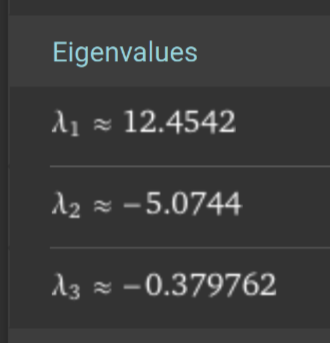
\includegraphics[width=0.3\textwidth]{eigenvalues.png}

		We found \underline{EVERY} eigenvalue!
	\end{center}
\end{frame}

\begin{frame}
	\frametitle{Is it good enough?}
	\begin{itemize}
		\item<1-> Similar convergence problems to Power Method: only guaranteed to work if $\left|\lambda_1\right|>\left|\lambda_2\right|>\ldots>\left|\lambda_n\right|$
		\item<2-> Needs modifications to find complex eigenvalues.
		\item<3-> Could be faster: runs in $\mathcal O(n^3)$ time for $n\times n$ matrix.
	\end{itemize}
\end{frame}

\begin{frame}
	\frametitle{Bad Example (1)}
	\begin{equation*}
		A=\begin{bmatrix}
			1 & 5 \\
			-1 & -3
		\end{bmatrix}
	\end{equation*}
	\begin{center}
		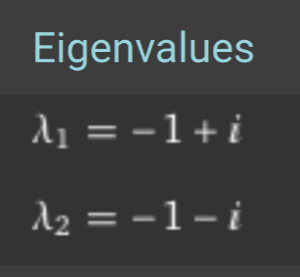
\includegraphics[width=0.25\textwidth]{eigenvalues2.png}
	\end{center}
	\vspace{-\abovedisplayskip}
	\onslide<2->{
	\begin{align*}
		\left|\lambda_1\right|
		&=\sqrt{(-1)^2+1^2}=\sqrt{2} \\
		\left|\lambda_2\right|
		&=\sqrt{(-1)^2+(-1)^2}=\sqrt{2}
	\end{align*}}
\end{frame}

\begin{frame}
	\frametitle{Bad Example (2)}
	\begin{center}
	\onslide<1->{
	\begin{minipage}{0.4\linewidth}
		\begin{align*}
			A_1 &= 
			\begin{bmatrix}
				1.00 & 5.00 \\
				-1.00 & -3.00 \\
			\end{bmatrix} \\
			A_2 &= 
			\begin{bmatrix}
				-3.00 & -5.00 \\
				1.00 & 1.00 \\
			\end{bmatrix} \\
			A_3 &= 
			\begin{bmatrix}
				-1.40 & 5.80 \\
				-0.20 & -0.60 \\
			\end{bmatrix} \\
			A_4 &= 
			\begin{bmatrix}
				-0.60 & -5.80 \\
				0.20 & -1.40 \\
			\end{bmatrix} \\
		\end{align*}
	\end{minipage}}
	\onslide<2->{
	\begin{minipage}{0.4\linewidth}
		\begin{align*}
			A_5 &= 
			\begin{bmatrix}
				1.00 & 5.00 \\
				-1.00 & -3.00 \\
			\end{bmatrix} \\
			A_6 &= 
			\begin{bmatrix}
				-3.00 & -5.00 \\
				1.00 & 1.00 \\
			\end{bmatrix} \\
			A_7 &= 
			\begin{bmatrix}
				-1.40 & 5.80 \\
				-0.20 & -0.60 \\
			\end{bmatrix} \\
			A_8 &= 
			\begin{bmatrix}
				-0.60 & -5.80 \\
				0.20 & -1.40 \\
			\end{bmatrix} \\
		\end{align*}
	\end{minipage}}

	\onslide<3->{
		$\displaystyle \lim_{k\to\infty}A_k$ will not converge onto a triangular matrix.
	}
	\end{center}
\end{frame}

\begin{frame}
	\frametitle{Another Bad Example}
	\vspace*{-\abovedisplayskip}
	\begin{gather*}
		\onslide<1->{A=\begin{bmatrix}
			0 & 0 & 0 & 1 \\
			0 & 0 & 1 & 0 \\
			0 & 1 & 0 & 0 \\
			1 & 0 & 0 & 0 \\
		\end{bmatrix}} \\
		\onslide<2->{
	    \lambda_1=1,
	    \lambda_2=-1,
	    \lambda_3=1,
		\lambda_4=-1} \\
		\onslide<3->{A_1=A=\underset{Q_1}{\begin{bmatrix}
			0 & 0 & 0 & 1 \\
			0 & 0 & 1 & 0 \\
			0 & 1 & 0 & 0 \\
			1 & 0 & 0 & 0 \\
		\end{bmatrix}}
		\underset{R_1}{\begin{bmatrix}
			1 & 0 & 0 & 0 \\
			0 & 1 & 0 & 0 \\
			0 & 0 & 1 & 0 \\
			0 & 0 & 0 & 1 \\
		\end{bmatrix}}
		=A_1I} \\
		\onslide<4->{A_2=R_1Q_1=IA_1=A_1}
	\end{gather*}
	\onslide<5->{This will never converge to a triangular matrix, since $A_i=A$ for all $i$.}
\end{frame}

\section{Improved $QR$ Algorithm}
\frame{\sectionpage}

\begin{frame}
	\frametitle{Improved $QR$ Algorithm}
	\begin{tcolorbox}[title={\textsc{Lapack} Algorithm},colback=red!5!white,colframe=red!75!black,parbox=false]
		\begin{enumerate}
			\item<1-> Reduce $A$ to an \textit{upper Hessenberg} form by calculating $A=QHQ^T$, where $Q$ is orthogonal and $H$ is an upper Hessenberg matrix. $H$ and $A$ are similar and share the same eigenvalues.
			\item<2-> Calculate the Schur form of $H$.
		\end{enumerate}
		\onslide<2->{Reference: \cite{lapack:eig}.}
	\end{tcolorbox}
	\onslide<3->{
		Used by the Linear Algebra PACKage (\textsc{Lapack}), which is used by NumPy and SciPy behind the scenes.
	}
\end{frame}

\begin{frame}
	\frametitle{References}
	\printbibliography
\end{frame}

\end{document}

